\chapter{Validation}
\label{ch:validation}

\section{Perfectly Stirred Reactor}

This non-dimensional problem aims to stress the species rate of formation source
term, our equations of state, and computation of energy.
The initial condition consists of a perfectly stirred mixture of \ce{H2}/\ce{O2}/\ce{AR}
with molar ratios $4$/$2$/$94$ at $T=1600$ \si{\kelvin} and $P=1$ atm. For this
configuration, Skinner et al. \cite{10.1063/1.1696266} expect an ignition delay of
$0.052$ \si{\milli\second}, characterized by [\ce{OH}] reaching $10^{-6}$ $\frac{\si{\mol}}{\si{\liter}}$.
As seen in Figure \ref{fig:skinner_perfect_reactor}, our results agree with theirs
within $1.3\%$ at $0.0513$ \si{\milli\second}. With the Cantera \cite{cantera} software
package, our relative error drops below $10^{-12}$ \%.

\begin{FigureInMulticol}
    \centering
    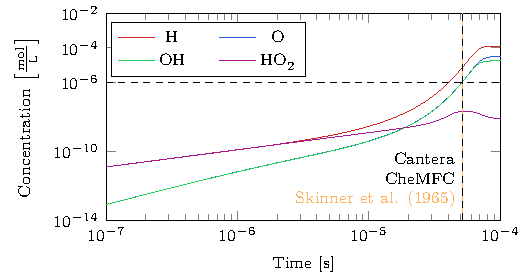
\includegraphics[width=\textwidth]{figures/nD_perfect_reactor/skinner.pdf}
    \captionof{figure}{Perfectly Stirred Reactor Ignition Delay}\label{fig:skinner_perfect_reactor}
\end{FigureInMulticol}

\section{Multi-species Inert Shock Tube}

Here, we aim to validate our shock-capturing capabilities and our implementation of
multi-species advection and convection, using a problem first described by Fedkiw
\cite{FedkiwPHD}, mentioned by Martínez-Ferrer et al. \cite{MARTINEZFERRER201488}.

The initial condition consists of $L=10$ \si{\centi\meter}-long tube discretized
with $400$ grid cells, containing a $2$/$1$/$7$ molar ratio of \ce{H2}/\ce{O2}/\ce{AR}.
The temperature and pressure are subject to a Riemann problem at $x=\frac{L}{2}$
whose left and right states are given, respectively, by
$\left(T_L,P_L\right) = (400\text{ \si{\kelvin}}, 8\text{ }000\text{ \si{\pascal}})$
and $\left(T_R,P_R\right) = (1\text{ }200\text{ \si{\kelvin}}, 80\text{ }000\text{ \si{\pascal}})$.
The left boundary is reflective while the right boundary is extrapolative.

We run the simulation for $t=40$ \si{\micro\second} using a constant step size of
$0.2$ \si{\micro\second}. Results are shown in Figure \ref{fig:1D_inert_shocktube}
against those of Fedkiw \cite{FedkiwPHD}. We also plot Martínez-Ferrer's
results for $\gamma$, the ratio of specific heat capacities, given the low resolution
of Fedkiw's data.

\begin{figure*}
    \begin{subfigure}[b]{0.5\textwidth}
        \centering
        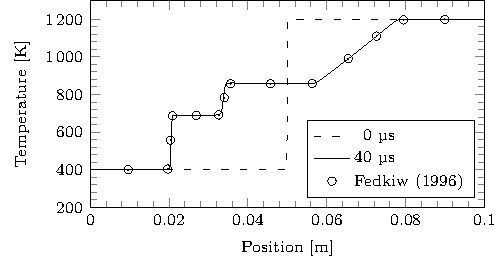
\includegraphics[width=\textwidth]{figures/1D_inert_shocktube/T.pdf}
        \caption{Temperature}
    \end{subfigure}
    \begin{subfigure}[b]{0.5\textwidth}
        \centering
        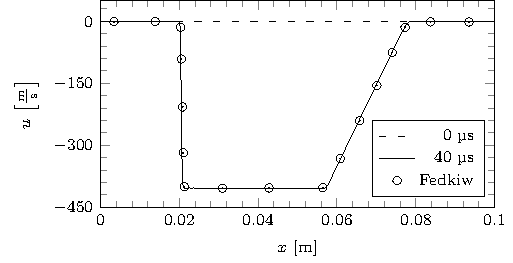
\includegraphics[width=\textwidth]{figures/1D_inert_shocktube/u.pdf}
        \caption{Velocity}
    \end{subfigure}
    \begin{subfigure}[b]{0.5\textwidth}
        \centering
        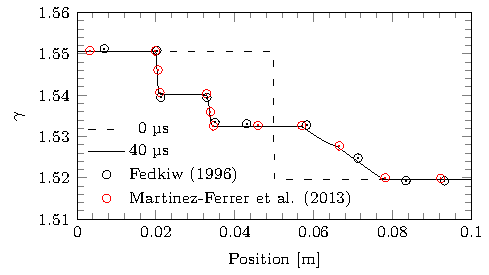
\includegraphics[width=\textwidth]{figures/1D_inert_shocktube/gamma.pdf}
        \caption{Ratio of Specific Heat Capacities}
    \end{subfigure}
    \begin{subfigure}[b]{0.5\textwidth}
        \centering
        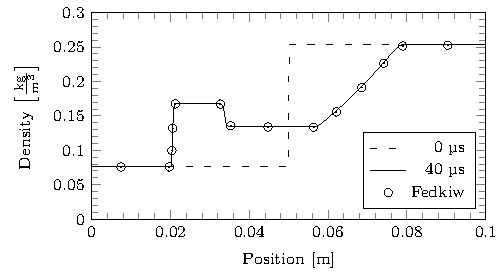
\includegraphics[width=\textwidth]{figures/1D_inert_shocktube/rho.pdf}
        \caption{Density}
    \end{subfigure}
    \caption{Multi-Species Inert Shock Tube. Temperature, Velocity, Ratio of Specific Heat Capacities, and Density profiles at $t=40$ \si{\micro\second}.}
    \label{fig:1D_inert_shocktube}
\end{figure*}

\section{Multi-Species Reactive Shock Tube}
\label{sec:1d_reactive_shocktube}

We now consider a reactive shock tube problem adapted by Martínez-Ferrer et al.
\cite{MARTINEZFERRER201488} to validate the interplay of advection, convection,
and chemical reactions while in the presence of discontinuities.

Initially, a $2$/$1$/$7$ molar ratio of \ce{H2}/\ce{O2}/\ce{AR} is placed in a
$L=12$ \si{\centi\meter}-long tube discretized with $400$ grid cells. A Riemann
problem is set at $x=\frac{L}{2}$ whose left and right states are given by,
respectively,
$\left(\rho_L,u_L,P_L\right) = \left(0.072\text{ }\frac{\si{\kilogram}}{\si{\meter}^3},0\text{ }\frac{\si{\meter}}{\si{\second}}, 7\text{ }173\text{ }\si{\pascal}\right)$
and
$\left(\rho_R,u_R,P_R\right) = \left(0.18075\text{ }\frac{\si{\kilogram}}{\si{\meter}^3},0\text{ }\frac{\si{\meter}}{\si{\second}}, 35\text{ }594\text{ }\si{\pascal}\right)$.
The left boundary is reflective while the right boundary is extrapolative.

When the leftward-moving wave reflects off the left boundary, it initiates a rightward-moving
reaction wave, pictured in Figure \ref{fig:1D_reactive_shocktube_Y}. We compare
our results to those of Martínez-Ferrer et al. \cite{MARTINEZFERRER201488}
in Figure \ref{fig:1D_reactive_shocktube_T_u}.

\begin{FigureInMulticol}
    \centering
    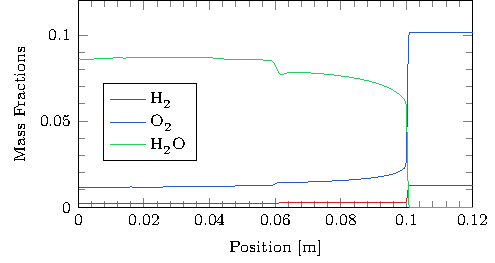
\includegraphics[width=\textwidth]{figures/1D_reactive_shocktube/Y.pdf}
    \captionof{figure}{
        Multi-Species Reactive Shock Tube. Mass Fraction profiles of \ce{H2}, \ce{O2}, and \ce{H2O}
        at $t=230$ \si{\micro\second}.
    }\label{fig:1D_reactive_shocktube_Y}
\end{FigureInMulticol}

\begin{figure*}
    \begin{subfigure}[b]{0.5\textwidth}
        \centering
        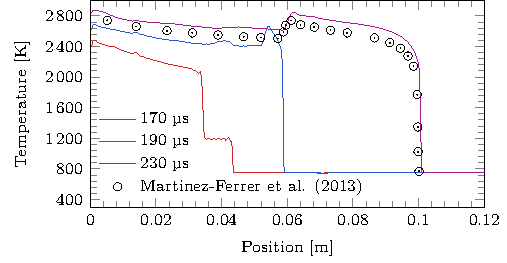
\includegraphics[width=\textwidth]{figures/1D_reactive_shocktube/T.pdf}
        \caption{Temperature}
    \end{subfigure}
    \begin{subfigure}[b]{0.5\textwidth}
        \centering
        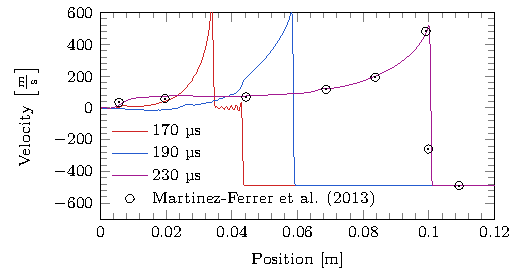
\includegraphics[width=\textwidth]{figures/1D_reactive_shocktube/u.pdf}
        \caption{Velocity}
    \end{subfigure}
    \caption{Multi-Species Reactive Shock Tube. Temperature and Velocity profiles at $t=170,190,230$ \si{\micro\second}.}
    \label{fig:1D_reactive_shocktube_T_u}
\end{figure*}
